%% Electronic Supplementary Information
\documentclass[10pt]{article}
\usepackage[a4paper,margin=2.2cm]{geometry}
\usepackage{mathptmx}
\usepackage[T1]{fontenc}
\usepackage{amsmath,amssymb,amsthm}
\usepackage{graphicx}
\usepackage{booktabs}
\usepackage[super,sort&compress,comma]{natbib}
\usepackage[font=small,labelfont=bf]{caption}
\usepackage{xcolor}
\usepackage{xr-hyper}
\usepackage[hidelinks]{hyperref}
\externaldocument[main-]{main}
\makeatletter\newcommand{\inputrows}[1]{\@@input #1 }\makeatother
\newcommand{\todo}[1]{\textcolor{red}{[#1]}}
\renewcommand{\thesection}{S\arabic{section}}
\renewcommand{\thetable}{S\arabic{table}}
\renewcommand{\thefigure}{S\arabic{figure}}
\renewcommand{\theequation}{S\arabic{equation}}
\newtheorem{proposition}{Proposition}
\renewcommand{\theproposition}{S\arabic{proposition}}
\raggedbottom
\newcommand{\Dcal}{\mathcal D_{\mathrm{cal}}}

\title{\bfseries Electronic Supplementary Information\\[4pt]
\large Conformal campaigns: engineering predictive uncertainty for chemical and materials screening}
\author{Petrus H. Zwart}
\date{}

\begin{document}
\maketitle
\tableofcontents

%% ------------------------------------------------------------------
\section{Notation and the outcome table}
\label{sec:notation}

The \emph{audit set} of the main text is a labelled random sample of the screened library used neither for training nor for calibration; in this document it is also called the test set.

Labels are $y\in\{0,1\}$: 1 for the in-class compounds, those with the property the screen looks for (toxic, soluble, or reaching the conductivity target), and 0 for the out-class compounds. The trained model gives predicted probabilities $\hat p(y\mid x)$ and nonconformity scores $s(x,y)=1-\hat p(y\mid x)$. For class $y$ let $S^{(y)}_{(1)}\le\dots\le S^{(y)}_{(n_y)}$ be the sorted scores of the $n_y$ calibration compounds of class $y$, and $\tau_y=S^{(y)}_{(k_y)}$. The prediction set is $C(x)=\{y: s(x,y)\le\tau_y\}$, one of $\{0\}$, $\{1\}$, $\{0,1\}$, $\varnothing$.

For a fixed pair of thresholds, write $c\in\{\{0\},\{1\},\{0,1\},\varnothing\}$ for the prediction set and
\begin{equation}
p_{y,c}=\Pr\big(Y=y,\ C(X)=c\big)
\end{equation}
for the probability of a cell of the outcome table (main text Table~\ref{main-tab:outcomes}) when compounds are independent. Under exchangeability we read $p_{y,c}$ as $p_{y,c}(Q)$, the long-run frequency of the cell given the de Finetti distribution $Q$ and the thresholds (Section~\ref{sec:intervals}). Any screening quantity is
\begin{equation}
p_g=\sum_{y,c} g(y,c)\,p_{y,c},\qquad g(y,c)\in\{0,1\},
\end{equation}
for a fixed indicator $g$ that selects cells. Examples: missed in-class compounds, $g=\mathbf 1\{y=1,c=\{0\}\}$; false leads, $g=\mathbf 1\{y=0,c=\{1\}\}$; deferred, $g=\mathbf 1\{c\in\{\{0,1\},\varnothing\}\}$; coverage, $g=\mathbf 1\{y\in c\}$. Ratios of such sums, for example the fraction of in-class compounds among compounds labelled $\{1\}$, follow directly. The same identity holds for counts: if $K_{y,c}$ is the number of test compounds in cell $(y,c)$, the count of quantity $g$ is $K_g=\sum_{y,c}g(y,c)K_{y,c}$. Within each class the cells sum to the class total, $\sum_c p_{y,c}=\Pr(Y=y)$.

%% ------------------------------------------------------------------
\section{Coverage given the calibration set and the finite-sample correction}
\label{sec:correction}

\paragraph{Exact laws.} Consider one class and drop the index $y$; let there be $n$ calibration scores and $\tau=S_{(k)}$, $u=n+1-k$; in this section $u$ denotes this grid index, not the predicted probability. Scores are assumed continuous. With tied scores, randomized tie-breaking restores all laws in this section exactly: every compound, calibration or future, receives an independent uniform number, and compounds are ordered by score and then by that number. This needs no knowledge of future scores. Our scripts implement it equivalently, on stored scores, by adding a uniform jitter smaller than the smallest gap between distinct scores. Without it, ties keep the one-sided coverage statement conservative, but they can break the two-sided count intervals of Sections~\ref{sec:intervals} and \ref{sec:calonly}: a cluster of tied scores at a threshold moves together, so the upper limit for the number of future compounds at or below the threshold can be exceeded (Section~\ref{sec:sim}, Table~\ref{tab:ties}). We therefore break ties at random in all molecular analyses. For a future batch of $m$ compounds of this class, the number whose score is at most $\tau$ depends only on the ranks of the $n+m$ exchangeable scores, all orderings of which are equally likely. Its distribution is therefore
\begin{equation}
\mathrm{BetaBinomial}(m;\,k,\,u),
\end{equation}
exactly and for any exchangeable data.\citep{Marques2025Beta} If compounds are independent with score distribution $F$, the coverage of the deployed model is $F(S_{(k)})$. This is the $k$-th order statistic of $n$ independent uniform variables, so
\begin{equation}
F(S_{(k)})\sim\mathrm{Beta}(k,\,n+1-k).
\end{equation}
This is Vovk's training-conditional result.\citep{Vovk2012PAC,Bian2023TrainingConditional} Under infinite exchangeability the same Beta law holds conditional on the de Finetti directing distribution, and therefore also marginally (Section~\ref{sec:intervals}).

\paragraph{Correction.} For a request $(\alpha,\delta)$ and batch size $m$, let $x^\star=\lceil(1-\alpha)m\rceil$, computed in integer arithmetic. The correction selects the least conservative order statistic, that is the largest $u$, such that
\begin{equation}
\Pr\big(X\ge x^\star\big)\ge 1-\delta,\qquad X\sim\mathrm{BetaBinomial}(m;\,n+1-u,\,u).
\end{equation}
The batch-free version replaces the Beta--Binomial by $\mathrm{Beta}(n+1-u,u)$ and the event by $\{Z\ge1-\alpha\}$. The procedure is applied separately to each class; for class $y$, $m$ is the number of future compounds of that class, and the guarantee holds conditional on the class labels.

\paragraph{Algorithm.} (i) Set $x^\star=\lceil(1-\alpha)m\rceil$. (ii) For $u=1,\dots,n$ compute the upper-tail probability above. (iii) Return the largest $u$ for which it is at least $1-\delta$, together with $k=n+1-u$ and the deployed level $u/(n+1)$; if there is none, return \emph{infeasible}.

\paragraph{Feasibility.} The most conservative choice $u=1$ gives coverage distributed as $\mathrm{Beta}(n,1)$. A batch-free request is therefore feasible if and only if
\begin{equation}
\alpha\ge1-\delta^{1/n}.
\end{equation}
A batch request is feasible if and only if $\Pr(X\ge x^\star)\ge1-\delta$ for $X\sim\mathrm{BetaBinomial}(m;\,n,\,1)$.
Distinct requests often select the same $u$ and hence the same deployed model (Fig.~\ref{fig:map}).

\paragraph{Baselines.} The standard choice is $k=\lceil(n+1)(1-\alpha)\rceil$. The DKW-based correction replaces $\alpha$ by $\alpha-\sqrt{\log(1/\delta)/(2n)}$ (one-sided bound with the Massart constant),\citep{Massart1990DKWM} and falls back to $k=n$ when this value is not positive.

\begin{figure}[ht]
\centering
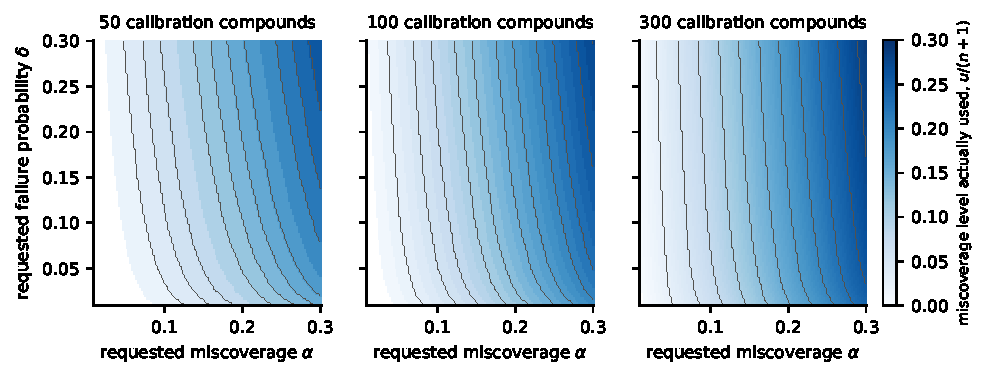
\includegraphics[width=0.85\textwidth]{figures/figS1_correction_map.pdf}
\caption{Deployed miscoverage level selected by the batch-free correction as a function of the request $(\alpha,\delta)$, for three calibration sizes. Contours mark deployed levels in steps of 0.025; white: infeasible requests ($\alpha<1-\delta^{1/n}$).}
\label{fig:map}
\end{figure}

\begin{table}[ht]
\centering
\caption{Fraction of calibration draws in which coverage over a batch of $m=100$ compounds fell below $90\%$ ($\alpha=\delta=0.10$; absolute Cauchy scores; $10^6$ draws). $u$: selected index; deployed level $u/(n+1)$. Theory (batch): Beta--Binomial value. Theory (batch-free): $\Pr(\text{coverage}<0.9)$ under the Beta law. DKW rows use the one-sided constant $\log(1/\delta)$. All rules were evaluated on the same draws. The batch-free correction selects the same $u$ as the batch correction for $n\le100$, and $u=10,15,19,23,41$ for $n=150,200,250,300,500$, with observed batch violation fractions 0.118, 0.168, 0.170, 0.171 and 0.212.}
\label{tab:grid}
\small
\begin{tabular}{rlrrrrr}
\toprule
$n$ & Threshold & $u$ & level & Observed & Theory (batch) & Theory (batch-free) \\
\midrule
\inputrows{tables/tab_grid_rows.tex}
\bottomrule
\end{tabular}
\end{table}

%% ------------------------------------------------------------------
\section{Prediction intervals for future-batch counts from a test set}
\label{sec:intervals}

\paragraph{Construction.} Fix the calibration set, hence the thresholds and the prediction-set map. For a fixed indicator $g$, let $I_1,\dots,I_n$ be its values on the test compounds and $I_{n+1},\dots,I_{n+m}$ on the future batch. Calibration, test and future compounds are jointly exchangeable, so given the calibration set the $n+m$ indicators are exchangeable. Let $K=\sum_{i\le n}I_i$, $K_m=\sum_{i>n}I_i$ and $T=K+K_m$. Conditional on $T=t$, every placement of the $t$ ones among the $n+m$ positions is equally likely, so
\begin{equation}
K\mid T=t\ \sim\ \mathrm{Hypergeometric}(n+m,\,t,\,n),
\end{equation}
whatever the distribution of the data. For each candidate $j$ for $K_m$, test $T=K+j$ with this distribution and keep $j$ if neither one-sided test rejects at level $\gamma/2$. The accepted values form an interval $[L,U]$ with $\Pr(L\le K_m\le U)\ge1-\gamma$.

\paragraph{Closed form.} For integers $0\le k\le n$ and $0\le j\le m$,
\begin{equation}
\Pr\big(K\ge k\mid T=k+j\big)=\Pr\big(B\le j\big),\qquad B\sim\mathrm{BetaBinomial}(m;\,k,\,n-k+1),
\end{equation}
and symmetrically for the other tail with parameters $(k+1,\,n-k)$.\citep{Thatcher1964} Hence
\begin{equation}
L=\min\{j:\ F_{\mathrm{BB}(m;k,n-k+1)}(j)>\gamma/2\},\qquad
U=\text{the }1-\gamma/2\text{ quantile of }\mathrm{BetaBinomial}(m;\,k+1,\,n-k),
\end{equation}
with $L=0$ if $k=0$ and $U=m$ if $k=n$. We verified both identities numerically for $n\in\{20,57,200\}$, $m\in\{10,100,1000\}$ and all $k$ and $j$; the largest discrepancy was $6\times10^{-13}$ (script in Section~\ref{sec:software}). The interval $[L,U]$ reaches at least $1-\gamma$ even conditional on each total $T$. It contains the Bayesian posterior predictive intervals with priors $\mathrm{Beta}(1,1)$ and $\mathrm{Beta}(1/2,1/2)$, so their coverage is never higher than that of the exact interval.

\paragraph{Sizing the audit set.} For planning, the exact limits are close to a normal approximation: for an outcome of frequency $p$, $n$ audit compounds and a batch of $m$, the 95\% interval for the future count is about $mp\pm2m\sqrt{p(1-p)(1/n+1/m)}$. The term $1/n$ is the uncertainty of the audited frequency and $1/m$ the variation of a finite batch; the second does not vanish however large the audit. For AqSolDB setting A ($p=0.23$ false leads, $n=384$, $m=1000$) the approximation gives $232\pm51$, against the exact $[183,285]$. Joint bounds over $J$ settings and $C$ outcomes replace the factor 2 by the corresponding normal quantile, about 3.8 for $JC=576$ and $\varepsilon=0.05$.

\paragraph{Target of the interval.} The interval covers the realized future count $K_m$; no fixed rate is assumed. If the compound source is regarded as infinitely exchangeable, de Finetti's theorem\citep{Aldous1985} gives a random distribution $Q$ such that, conditional on $Q$, compounds are independent draws from $Q$. Conditional on $Q$ and the calibration set the test indicators are then independent Bernoulli variables with success probability
\begin{equation}
p_g(Q)=\Pr_Q\big(g(Y,C(X))=1\big),
\end{equation}
so $K$ is Binomial and the Clopper--Pearson interval covers $p_g(Q)$ with probability at least $1-\gamma$, conditionally and therefore marginally. $p_g(Q)$ is the long-run frequency of the outcome in this deployment. The probability $\Pr(g=1\mid\Dcal)$, averaged over $Q$, is not the success probability of independent trials, and intervals for it are not valid in general; in the two-stage simulation of Table~\ref{tab:twostage} Clopper--Pearson coverage of that quantity fell to 73\%. Finite exchangeable sequences need not be mixtures of independent sequences;\citep{DiaconisFreedman1980} the hypergeometric construction above does not need this representation.

\paragraph{Several outcomes.} Each interval is valid for one indicator fixed before seeing the test set. For $J$ indicators, intervals at level $\gamma/J$ hold simultaneously. A joint region for the full outcome table can be obtained from the multivariate hypergeometric distribution of the cell counts given their totals.


%% ------------------------------------------------------------------
\section{Prediction intervals from the calibration set alone}
\label{sec:calonly}

\paragraph{Events.} Use the notation of Section~\ref{sec:geometry}: $u=\hat p(1\mid x)$, $0\in C(x)$ iff $u\le\tau_0$, and $1\in C(x)$ iff $u\ge1-\tau_1$. Here $\tau_0$ is the $k_0$-th smallest of the $n_0$ out-class calibration scores $u$, and $\tau_1$ is the $k_1$-th smallest of the $n_1$ in-class calibration scores $1-u$. For out-class compounds define
\begin{equation}
A_0=\{u\le\tau_0\}\ \text{(coverage)},\qquad B_0=\{u\ge1-\tau_1\}\ \text{(labelled in-class)},
\end{equation}
and for in-class compounds $A_1=\{u\ge1-\tau_1\}$ and $B_1=\{u\le\tau_0\}$.

\paragraph{Own-class events.} Let $m_y$ be the number of future compounds of class $y$. The number of them in $A_y$ is the number of $m_y$ exchangeable scores at or below the $k_y$-th of $n_y$ calibration scores. Its distribution is exactly\citep{Marques2025Beta}
\begin{equation}
\mathrm{BetaBinomial}(m_y;\,k_y,\,n_y+1-k_y),
\end{equation}
and its equal-tailed quantiles give an interval.

\paragraph{Cross-class events.} $B_0$ depends on the data only through $\tau_1$, which is a function of the in-class calibration compounds. Given the labels and the in-class calibration compounds, the out-class calibration compounds and the future out-class compounds are exchangeable. Let $c_0$ be the number of out-class calibration compounds in $B_0$. The test-set construction of Section~\ref{sec:intervals}, with $n=n_0$, $K=c_0$ and $m=m_0$, then gives an interval for the number of future out-class compounds in $B_0$. The same holds for $B_1$ with the roles of the classes exchanged.

\paragraph{Cells.} By Proposition~\ref{prop:regimes}, if $\tau_0+\tau_1\ge1$ then $A_0^c\subseteq B_0$, and the out-class row is
\begin{equation}
\{1\}=A_0^c,\qquad \{0\}=B_0^c,\qquad \text{both}=A_0\cap B_0,\qquad \varnothing=\emptyset .
\end{equation}
If $\tau_0+\tau_1<1$ then $A_0\cap B_0=\emptyset$, and
\begin{equation}
\{0\}=A_0,\qquad \{1\}=B_0,\qquad \varnothing=A_0^c\cap B_0^c,\qquad \text{both}=\emptyset .
\end{equation}
The regime is known once the thresholds are set, but it depends on the calibration data of both classes, so a cell's identity with one event or the other is data dependent. We therefore compute the interval for $|A_0|$ (rank law) and the interval for $|B_0|$ (cross-class) each at level $1-\gamma/2$. Both then hold simultaneously with probability at least $1-\gamma$, whatever the regime. Every cell of the row is bounded by arithmetic on the two: in the two-label regime, $\{1\}$ and $\{0\}$ are bounded by the complements of $A_0$ and $B_0$, and the both-labels cell by $|A_0|+|B_0|-m_0$; in the empty regime, $\{0\}$ and $\{1\}$ are bounded by $A_0$ and $B_0$, and the empty cell by $m_0-|A_0|-|B_0|$. The intervals for all cells of the row hold jointly at level $1-\gamma$. The in-class row is analogous: missed in-class compounds are $A_1^c$ (rank law) and confident hits are $B_1^c$ (cross-class) in the two-label regime.

\paragraph{Mixed batches.} The guarantees above are conditional on $m_y$. For a batch of $m$ compounds of unknown composition, the number of in-class compounds $m_1$ has the test-set interval from the calibration class counts ($K=n_1$ out of $n_0+n_1$). We compute the interval for $m_1$ at level $1-\gamma/2$, and each of the four event intervals ($A_0,B_0,A_1,B_1$) at level $1-\gamma/8$, for every $m_1$ in that interval, and take the union over $m_1$. By the union bound the five statements hold together with probability at least $1-\gamma$, so the intervals for all cells of the mixed batch hold jointly at level $1-\gamma$. The union over $m_1$ is conservative; mixing the class-wise laws over the exact distribution of $m_1$ would give shorter intervals.

\paragraph{When it does not apply.} If scores are not class probabilities ($s(x,0)+s(x,1)\ne1$), the sets $A_0\cap B_0$ and $A_0^c\cap B_0^c$ can both have positive probability. Their counts then depend on the joint behaviour of two thresholds on the same compounds, and a test set is needed. Evaluating a class's own threshold on the compounds that set it, beyond the rank law, is not allowed (Section~\ref{sec:reuse}).

\paragraph{Validation.} Table~\ref{tab:calonly} reports coverage and width from the simulation of Section~\ref{sec:sim}.

\begin{table*}[ht]
\centering
\caption{Calibration-only intervals (nominal 95\%), future batch of $m=1000$. Class-conditional: coverage of the row intervals given the number of future compounds of the class. Mixed: coverage for a batch of unknown composition (union over the interval for the number of in-class; levels as in Section~\ref{sec:calonly}). Widths are for the mixed batch. Split budget: the same $n$ labelled compounds split equally into calibration and audit sets, with audit-set intervals. $n=300$: 2897 replicates (103 skipped with fewer than 20 calibration compounds in a class), all mixed-batch cells covered together in 99.7\%; $n=1000$: 3000 replicates (0 skipped with fewer than 20 calibration compounds in a class), all mixed-batch cells covered together in 99.5\%.}
\label{tab:calonly}
\small
\begin{tabular}{rlccrrc}
\toprule
$n$ & Cell & \multicolumn{2}{c}{Coverage, calibration only} & \multicolumn{2}{c}{Mean width} & Coverage \\
 & & class-conditional & mixed & calibration only & split budget & split budget \\
\midrule
300 & out-class $\{0\}$ (correct rejection) & 0.978 & 1.000 & 202.9 & 158.7 & 0.964 \\
 & out-class $\{1\}$ (false lead) & 0.977 & 0.999 & 78.9 & 69.4 & 0.972 \\
 & out-class deferred & 0.999 & 1.000 & 180.7 & 106.2 & 0.973 \\
 & in-class $\{1\}$ (confident hit) & 0.981 & 0.999 & 164.8 & 138.8 & 0.965 \\
 & in-class $\{0\}$ (missed in-class) & 0.989 & 0.999 & 47.8 & 42.1 & 0.988 \\
 & in-class deferred & 0.998 & 1.000 & 104.8 & 68.8 & 0.982 \\
\midrule
1000 & out-class $\{0\}$ (correct rejection) & 0.979 & 1.000 & 138.9 & 99.7 & 0.960 \\
 & out-class $\{1\}$ (false lead) & 0.984 & 0.999 & 52.9 & 43.7 & 0.972 \\
 & out-class deferred & 1.000 & 1.000 & 123.7 & 59.8 & 0.969 \\
 & in-class $\{1\}$ (confident hit) & 0.981 & 0.998 & 111.2 & 85.2 & 0.946 \\
 & in-class $\{0\}$ (missed in-class) & 0.987 & 0.999 & 31.8 & 24.8 & 0.977 \\
 & in-class deferred & 1.000 & 1.000 & 71.3 & 36.9 & 0.976 \\
\bottomrule
\end{tabular}
\end{table*}


%% ------------------------------------------------------------------
\section{Same-class reuse of the calibration set, and the leave-one-out estimate}
\label{sec:reuse}

Let $I_i(t)=\mathbf 1\{S_i\le t\}$ for the $n$ calibration scores of one class. If $\tau=S_{(k)}=t$, then exactly $k$ indicators equal one, so the indicators are not independent given the threshold:
\begin{equation}
\mathrm{Cov}\big(I_i(t),I_j(t)\mid\tau=t\big)=-\frac{k(n-k)}{n^2(n-1)}<0,\qquad i\ne j,\ k<n.
\end{equation}
Outcome counts that evaluate a class's own threshold on the calibration compounds of that class inherit this dependence and are not exchangeable with future counts; only the rank law of Section~\ref{sec:correction} describes them exactly. Cross-class events are not affected (Section~\ref{sec:calonly}). Intervals built from them are too narrow, and their centres can also be biased near thresholds.

\paragraph{Leave-one-out estimate.} When no test set is available, each calibration compound $i$ can be assigned to a prediction set using thresholds recomputed without it. The pooled cell counts give a leave-one-out estimate of the outcome table.\citep{vovk2015crossconformal,barber2021predictive} The thresholds change from one compound to the next, so this estimate carries no guarantee. With class probabilities, the calibration-only intervals of Section~\ref{sec:calonly} make it unnecessary; for other scores it is useful only for exploring settings before a test set is collected.

%% ------------------------------------------------------------------
\section{Binary prediction sets with probability scores}
\label{sec:geometry}

Write $u=s(x,0)=\hat p(1\mid x)$. If $\hat p(0\mid x)+\hat p(1\mid x)=1$ then $s(x,1)=1-u$, and the sets are determined by $u$ alone: $0\in C(x)$ iff $u\le\tau_0$ and $1\in C(x)$ iff $u\ge1-\tau_1$.

\begin{proposition}
\label{prop:regimes}
With probability scores, (i) the two-label set has positive probability only if $\tau_0+\tau_1>1$, in which case $u\in[1-\tau_1,\tau_0]$; (ii) the empty set has positive probability only if $\tau_0+\tau_1<1$, in which case $u\in(\tau_0,1-\tau_1)$; (iii) if $\tau_0+\tau_1=1$ (and $u$ has a continuous distribution) only single-label sets occur.
\end{proposition}
\begin{proof}
Direct from the two conditions on $u$.
\end{proof}

When $\tau_0+\tau_1>1$, compounds with $u<1-\tau_1$ receive $\{0\}$, those with $u>\tau_0$ receive $\{1\}$, and those in between receive both labels (main text Fig.~\ref{main-fig:sets}). Raising $\tau_1$ moves compounds from $\{0\}$ to both labels; raising $\tau_0$ moves compounds from $\{1\}$ to both labels. Each single-label set is thus controlled by the threshold of the other class. This is why changing the request for one class can change the outcomes of the other.

%% ------------------------------------------------------------------
\section{Cost ratios for which acting on single labels is cheapest}
\label{sec:costs}

Consider actions: label 0, label 1, or defer, with costs $c_{\text{miss}}$ for assigning 0 to a compound of class 1, $c_{\text{lead}}$ for assigning 1 to a compound of class 0, $c_{\text{defer}}$ for deferring, and zero for correct labels. For a prediction set $c$ with positive probability let
\begin{equation}
\eta_c=\Pr\big(Y=1\mid C(X)=c\big)=\frac{p_{1,c}}{p_{0,c}+p_{1,c}}.
\end{equation}
A rule that acts only on the prediction set has expected costs $\eta_c c_{\text{miss}}$ (label 0), $(1-\eta_c)c_{\text{lead}}$ (label 1) and $c_{\text{defer}}$ (defer). With $\lambda=c_{\text{miss}}/c_{\text{lead}}$ and $\rho=c_{\text{defer}}/c_{\text{lead}}$, the rule ``$\{1\}\to$ label 1, $\{0\}\to$ label 0, otherwise defer'' minimizes expected cost if and only if all of the following hold for the sets that occur:\citep{Chow1970}
\begin{equation}
\eta_{\{1\}}\ge\max\Big\{\frac{1}{1+\lambda},\,1-\rho\Big\},
\end{equation}
\begin{equation}
\eta_{\{0\}}\le\min\Big\{\frac{1}{1+\lambda},\,\frac{\rho}{\lambda}\Big\},
\end{equation}
\begin{equation}
\frac{\rho}{\lambda}\le\eta_c\le1-\rho\quad\text{for } c\in\{\{0,1\},\varnothing\}.
\end{equation}
Each condition is linear in $(\lambda,\rho)$, so the admissible region is a polygon, possibly empty. Deferral can be optimal only if $c_{\text{defer}}\le c_{\text{miss}}c_{\text{lead}}/(c_{\text{miss}}+c_{\text{lead}})$. The $\eta_c$ are estimated from the outcome table.

\paragraph{Set-based rules contain Chow's rule.} Let $\eta(u)=\Pr(Y=1\mid u)$, and suppose $\eta$ is nondecreasing in $u$, as it is when the model ranks compounds sensibly. In units of $c_{\text{lead}}$, the expected costs of the three actions for a compound with score $u$ are $\lambda\eta(u)$ (label 0), $1-\eta(u)$ (label 1) and $\rho$ (defer). Chow's optimal rule\citep{Chow1970} takes the cheapest action at each $u$. Because $\eta$ is monotone, the optimal rule labels 0 for $u<l$, defers for $l\le u\le h$ and labels 1 for $u>h$, for some $l\le h$. The set-based rule with $\tau_0=h$ and $\tau_1=1-l$ produces exactly this partition (Section~\ref{sec:geometry}). If deferral is never optimal, then $l=h$ and the thresholds satisfy $\tau_0+\tau_1=1$. Conformal thresholds are calibration order statistics, so $(l,h)$ can be matched only up to the spacing of the calibration scores. In addition, a sweep over a finite grid of requests reaches only the threshold pairs on that grid. Choosing the request by cost therefore loses nothing relative to Chow's rule beyond the resolution of the calibration scores and of the request grid, \emph{provided} $\eta$ is monotone. Requiring coverage of at least $1-\alpha$ for both classes restricts $(l,h)$, and its cost can be computed (Table~\ref{tab:cost}). The argument needs $\eta$ to be monotone, not calibrated: the set-based rule uses only the ordering of $u$. If $\eta$ is not monotone, Chow's rule on calibrated probabilities is not a two-threshold rule on $u$ and can be cheaper; Table~\ref{tab:tox21mono} gives a monotonicity diagnostic for the Tox21 models. The containment is a statement about population rules. On finite data, a set rule chosen from calibration estimates and Chow's rule on fitted probabilities are both estimates, and either can be cheaper (Table~\ref{tab:chow}). What the set rule adds is the interval guarantee for its outcome counts, which after selection holds only with the correction of the Selection paragraph below.

\paragraph{Uncertainty in $\eta_c$.} The conditions above use estimated within-set fractions $\hat\eta_c$. A robust region is the set of $(\lambda,\rho)$ for which the conditions hold for every $\eta_c$ in simultaneous Clopper--Pearson intervals: Bonferroni over the sets that occur, computed from the counts $p_{0,c},p_{1,c}$ of the outcome table. The conditions are monotone in each $\eta_c$, so this needs only the interval endpoints. These intervals need the joint counts of label and prediction set on compounds not used to set the thresholds, that is a labelled test set; the calibration-only intervals of Section~\ref{sec:calonly} bound the cells of each row separately and do not by themselves give intervals for the within-set fractions. In the solubility example the robust region therefore uses the test set.

\paragraph{Selection.} A sweep over a grid of $J$ requests yields at most $J$ distinct rules. If intervals for all rules are computed at level $\gamma/J$, they hold simultaneously with probability at least $1-\gamma$, so the intervals of any rule chosen by looking at them remain valid. Choosing by an estimated cost or by a capacity constraint is then safe. We divide by the size of the request grid, which is fixed in advance; dividing by the number of distinct rules is also valid when the thresholds are set from data independent of the data used for the intervals (as in the test-set design), because the set of distinct rules is then fixed given the calibration set. Bonferroni is conservative when $J$ is large. Sequential procedures such as fixed-sequence testing\citep{Angelopoulos2021LTT} control error for hypotheses about fixed parameters, for example the long-run deferral rate $p_g(Q)$ of Section~\ref{sec:intervals}; they do not by themselves protect statements about realized future counts, because which settings exceed a capacity in the future batch is itself random. We therefore use Bonferroni for all statements about future counts.

\paragraph{The usual set-to-action rule is max--min optimal.} Measure costs in units of a false lead: a miss costs $\lambda$, a deferral $\rho$, a correct call 0. Kiyani \textit{et al.}\ show that a decision maker who knows only a prediction set with marginal coverage, and wants a high-probability guarantee on its utility, should take the action with the best worst case over the labels in the set.\citep{Kiyani2025RAC} For $\{1\}$ the worst-case cost of labelling 1 is 0, so the rule labels 1; likewise for $\{0\}$. For $\{0,1\}$ the worst cases are $\lambda$ (label 0), 1 (label 1) and $\rho$ (defer), so the rule defers whenever $\rho\le\min(\lambda,1)$. Empty sets occur here by design rather than only on miscoverage; we defer them. Acting on single labels and deferring the rest is therefore the max--min action for every cost with $\rho\le\min(\lambda,1)$, whatever the coverage setting. Expected-cost (Chow) optimality, the criterion that governs the average over a campaign, holds only where the within-set fractions satisfy the conditions above; the two criteria answer different questions. Kiyani \textit{et al.}\ also show that, for a given utility, the optimal prediction sets are level sets of utility rather than of a score, so class-conditional threshold sets are not in general the optimal sets.

\paragraph{Scenario maps (main text Fig.~\ref{main-fig:solubility}, Fig.~\ref{fig:calisolscen}).} For one split, each request on the $12\times12$ grid ($\delta=0.10$, batch correction with planned class counts) sets thresholds on the calibration set. For a future batch of $M=1000$, the audit set gives the point estimate of each outcome count and a one-sided bound from the construction of Section~\ref{sec:intervals}: upper bounds for deferrals (measurements), false leads and missed in-class compounds, a lower bound for confirmed in-class compounds. Each bound is computed at level $\varepsilon/(JC)$ with $\varepsilon=0.05$, $J=144$ requests and $C=4$ bounded outcomes ($8.7\times10^{-5}$), so that all bounds of all requests hold together with probability at least 95\%. A scenario lists limits on some of these bounds; a request is feasible if all its bounds satisfy the limits, and the feasible request with the fewest expected false leads is chosen. Because every bound of every request holds together, the chosen setting satisfies its constraints with probability at least 95\% although it was chosen by looking at the audit set. The CALiSol-23 maps use the first random split of the electrolyte screen. If the objective and the limits are monotone in the outcomes, an optimal feasible setting lies on the Pareto front of the vectors (upper bounds on deferrals, false leads and missed in-class compounds; lower bound on confirmed in-class compounds; and, for the point objective, expected false leads): if setting $b$ dominates setting $a$, then $b$ meets every limit $a$ meets and is at least as good under the objective. On these maps the front held 105 of 144 distinct settings for AqSolDB and 33 of 107 for CALiSol-23, and the chosen setting lay on it in all four scenarios; adding the expected false leads to the vector did not change the front. For the electrolyte screen (Fig.~\ref{fig:calisolscen}), with at most 200 measurements per 1000, at least 60 confirmed good electrolytes and at most 40 missed, 56 of 144 requests were feasible; halving the measurement budget left 19 and raised the expected false leads of the best setting from 53 to 67 per 1000. Because deferrals arise from both-label sets for some requests and from empty sets for others, the measurement constraint bounds the feasible region from two sides. For AqSolDB, 23--48 settings per split were expected-cost optimal for some cost ratio on the grid of Fig.~\ref{fig:costmap}, and the ratios for which acting on the sets stays optimal over the uncertainty of the within-set fractions covered 1--6\% of the grid; the choice by constraints in the main text needs no cost ratio.

\begin{figure}[ht]
\centering
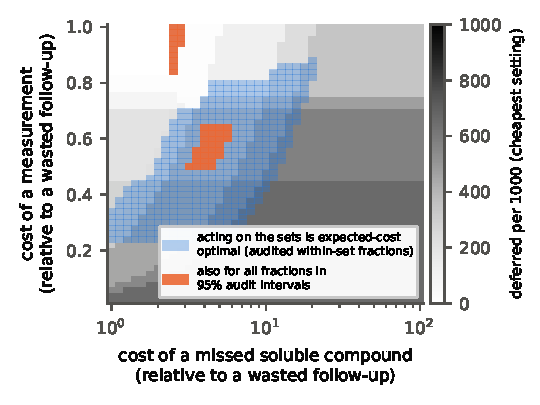
\includegraphics[width=0.62\textwidth]{figures/figS2_costmap.pdf}
\caption{AqSolDB lipophilic screen (split 0): for each pair of cost ratios, the number of deferrals of the setting with the lowest expected cost (grey), computed from audited counts. Blue: cost ratios for which acting on single labels and deferring the rest is expected-cost optimal for that setting at the audited within-set fractions. Orange: where this holds for all fractions within simultaneous 95\% audit intervals. Regions are evaluated cell by cell.}
\label{fig:costmap}
\end{figure}

\begin{figure}[ht]
\centering
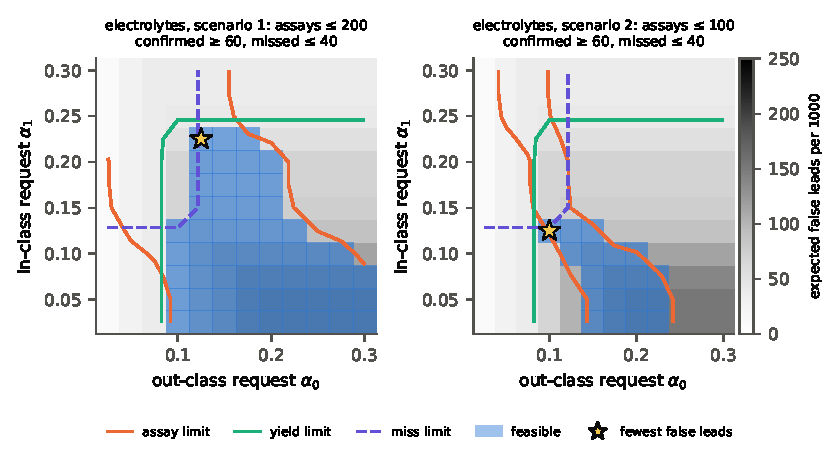
\includegraphics[width=0.85\textwidth]{figures/figS3_calisol_scenarios.pdf}
\caption{Scenario maps for the electrolyte screen (CALiSol-23, first random split), as in main text Fig.~\ref{main-fig:solubility}. Left: at most 200 measurements, at least 60 confirmed good electrolytes and at most 40 missed per 1000. Right: at most 100 measurements. The measurement limit bounds the feasible region on two sides because deferrals come from both-label sets for some requests and from empty sets for others.}
\label{fig:calisolscen}
\end{figure}

\begin{table}[ht]
\centering
\caption{Expected cost relative to Chow's optimal rule (\%), constrained (coverage $\ge0.90$ for both classes) / default ($\alpha=0.10$ for both classes). $\lambda$: cost of a miss; $\rho$: cost of an assay; both relative to a false lead.}
\label{tab:cost}
\small
\begin{tabular}{llrrrr}
\toprule
Scores & $\lambda$ & $\rho=0.1$ & $\rho=0.3$ & $\rho=0.5$ & $\rho=0.8$ \\
\midrule
well separated & 2 & 0 / 35 & 0 / 38 & 0 / 68 & 0 / 138 \\
 & 5 & 0 / 23 & 0 / 12 & 0 / 25 & 0 / 58 \\
 & 10 & 0 / 27 & 0 / 2 & 0 / 7 & 0 / 26 \\
 & 20 & 0 / 48 & 0 / 3 & 0 / 0 & 0 / 9 \\
 & 50 & 0 / 119 & 0 / 26 & 0 / 9 & 0 / 5 \\
\midrule
overlapping & 2 & 0 / 134 & 4 / 41 & 18 / 31 & 47 / 47 \\
 & 5 & 0 / 152 & 0 / 31 & 0 / 9 & 6 / 5 \\
 & 10 & 0 / 220 & 0 / 49 & 0 / 15 & 0 / 1 \\
 & 20 & 0 / 372 & 0 / 100 & 0 / 44 & 0 / 16 \\
 & 50 & 0 / 838 & 0 / 262 & 0 / 144 & 0 / 80 \\
\midrule
balanced, overlapping & 2 & 0 / 132 & 0 / 21 & 1 / 5 & 14 / 14 \\
 & 5 & 0 / 319 & 0 / 91 & 1 / 48 & 12 / 35 \\
 & 10 & 0 / 632 & 0 / 212 & 1 / 127 & 10 / 89 \\
 & 20 & 0 / 1259 & 0 / 453 & 1 / 287 & 9 / 203 \\
 & 50 & 0 / 3133 & 0 / 1171 & 0 / 762 & 8 / 543 \\
\bottomrule
\end{tabular}
\end{table}


%% ------------------------------------------------------------------
\section{Simulation protocols and additional results}
\label{sec:sim}

\paragraph{Threshold correction (main text Table~\ref{main-tab:correction}, Table~\ref{tab:grid}).} Calibration scores were drawn from the absolute value of a Cauchy distribution, and the future batch ($m=100$) from the same distribution, for $10^6$ independent calibration draws per $n$; all threshold rules were evaluated on the same draws.

\paragraph{Prediction intervals (main text Fig.~\ref{main-fig:validation}).} Each replicate drew a data distribution $Q$: prevalence $\pi\sim\mathrm{U}(0.05,0.5)$; predicted probability of being in-class $\mathrm{Beta}(a_1,b_1)$ for in-class compounds with $a_1\sim\mathrm U(2,10)$, $b_1\sim\mathrm U(2,4)$; and $\mathrm{Beta}(a_0,b_0)$ for out-class compounds with $a_0\sim\mathrm U(1.5,3)$, $b_0\sim\mathrm U(5,9)$. It then drew 1000 calibration compounds, $n$ test compounds and $m=1000$ future compounds independently from $Q$. Over replicates the data are exchangeable but not independent. Thresholds used the batch-free correction with $\alpha=\delta=0.10$ for each class. Replicates with fewer than 30 calibration compounds in a class were skipped (none occurred). The long-run cell probabilities given $Q$ and the thresholds were computed exactly from the Beta distribution functions. Besides the audit interval, three common alternatives were evaluated: the Bayesian posterior predictive with a uniform prior, Beta--Binomial$(m;K+1,n-K+1)$; the plug-in interval, Binomial$(m,K/n)$ quantiles; and $m$ times the Clopper--Pearson interval for the rate, rounded outward. Results are in Table~\ref{tab:validation}. Because the data are independent given $Q$, this design does not separate validity under exchangeability from validity under independence. The future count varies for two reasons: the audited rate is uncertain, which adds a variance of about $m^2p(1-p)/n$, and the batch itself is a sample, which adds about $mp(1-p)$. The plug-in interval keeps only the second term and is too narrow by a factor of about $\sqrt{1+m/n}$; $m$ times the Clopper--Pearson interval keeps only the first and is too narrow by about $\sqrt{1+n/m}$. Each fails where the term it omits dominates: the plug-in for small audits, the scaled Clopper--Pearson interval for audits as large as the batch, and for any audit when the batch is small. The audit interval accounts for both terms. Its limits use the same Beta parameters as the Clopper--Pearson limits but take Beta--Binomial rather than Beta quantiles, and as $m\to\infty$, $K_m/m$ recovers the Clopper--Pearson interval for the rate.

\paragraph{Calibration-only intervals (main text Fig.~\ref{main-fig:calonly}, Table~\ref{tab:calonly}).} Data distributions as above; row-simultaneous intervals as described in Section~\ref{sec:calonly}; $n\in\{300,1000\}$ calibration compounds; batch-free correction with $\alpha=\delta=0.10$; future batch $m=1000$; 3000 replicates, of which those with fewer than 20 calibration compounds in a class were skipped (103 at $n=300$, none at $n=1000$). Class-conditional coverage was evaluated given the realized $m_y$, and mixed-batch coverage with the union over $m_1$. The comparison spends the same budget of $n$ labelled compounds half on calibration and half on a test set, and computes test-set intervals for the mixed batch.

\paragraph{Cost (main text Table~\ref{main-tab:cost}, Table~\ref{tab:cost}).} Exact population computation, with out-class scores $u\sim\mathrm{Beta}(2,7)$ and in-class scores $u\sim\mathrm{Beta}(a,b)$. The three settings are prevalence 0.15 with $(9,3)$ (well separated), prevalence 0.15 with $(4,3)$ (overlapping), and prevalence 0.5 with $(4,3)$ (balanced, overlapping). Thresholds $(l,h)$ were searched on a grid of 801 points. Chow: minimum over all $l\le h$. Constrained: minimum subject to class-wise coverage $\ge0.90$. Default: both coverages exactly 0.90.

\paragraph{Selection.} 4000 replicates. In each, prevalence $\sim\mathrm U(0.1,0.4)$, in-class compounds $\mathrm{Beta}(a,b)$ with $a\sim\mathrm U(3,9)$ and $b\sim\mathrm U(2,4)$, out-class compounds $\mathrm{Beta}(2,7)$. There were 500 calibration compounds, 200 test compounds and a future batch of 1000. The candidates were the rules from the standard thresholds at $\alpha_0,\alpha_1\in\{0.02,\dots,0.30\}$ (10 values each), de-duplicated to distinct threshold pairs (median 100, range 90--100). The rule chosen was the one with the fewest test-set errors (missed in-class compounds plus false leads) among the rules whose one-sided upper limit for deferrals was at most 150. The level of this check was set either at $0.05$ for each rule (unadjusted) or at $0.05/J$ with $J$ the number of distinct rules (Bonferroni). For the chosen rule we recorded whether its realized future deferrals exceeded capacity, and whether its two-sided error interval, at the same per-rule level, covered its realized future errors. A rule was found in every replicate. Capacity was exceeded in 0.47\% of replicates (unadjusted) and 0.03\% (Bonferroni), against the nominal 5\%. The chosen rules made 43.5 and 52.5 future errors per batch of 1000. The error interval of the chosen rule covered the realized errors in 95.6\% (unadjusted) and 100\% (Bonferroni) of replicates. In this design the selection effect on the chosen rule's intervals is small, because neighbouring rules have strongly correlated counts; the unadjusted procedure carries no guarantee nonetheless.

\paragraph{Tied scores (Table~\ref{tab:ties}).} Out-class scores were drawn from $\mathrm{Beta}(2,7)$ and in-class scores from $\mathrm{Beta}(6,3)$, prevalence 0.2, with 1000 calibration and 1000 future compounds. A fraction $t\in\{0,4,6,10\}\%$ of out-class compounds, in both sets, received one common score at the 0.92 quantile of the out-class distribution. Thresholds were standard at $\alpha=0.10$, and the class-conditional calibration-only intervals of Section~\ref{sec:calonly} were evaluated with ties kept or broken at random. With ties kept, coverage of the correct-rejection count fell from 0.98 to 0.86, 0.81 and 0.71 for $t=4$, 6 and 10\%, and coverage of the whole out-class row to 0.84, 0.79 and 0.67. With randomized tie-breaking, coverage was at least 0.97 for every cell and at least 0.96 for each row. Tox21 out-class compounds have 3--4\% tied scores (Table~\ref{tab:batchlaw}).

\begin{table}[ht]
\centering
\caption{Tied scores and calibration-only intervals ($n=1000$ calibration and $m=1000$ future compounds, prevalence 0.2, standard thresholds at $\alpha=0.10$; 2000 replicates per row). A fraction of out-class compounds share one score at the 0.92 quantile of the out-class distribution, as for a cluster of identical fingerprints. Entries: coverage of the nominal 95\% class-conditional intervals, with ties kept (kept) and with randomized tie-breaking (rand.). Row: all cells of the class row covered together.}
\label{tab:ties}
\small
\begin{tabular}{rrrrrrrrr}
\toprule
Tied & \multicolumn{2}{c}{correct rejection} & \multicolumn{2}{c}{false lead} & \multicolumn{2}{c}{out-class row} & \multicolumn{2}{c}{in-class row} \\
out-class (\%) & kept & rand. & kept & rand. & kept & rand. & kept & rand. \\
\midrule
0 & 0.980 & 0.974 & 0.980 & 0.981 & 0.966 & 0.963 & 0.975 & 0.972 \\
4 & 0.857 & 0.983 & 0.969 & 0.982 & 0.838 & 0.971 & 0.976 & 0.977 \\
6 & 0.811 & 0.981 & 0.967 & 0.981 & 0.787 & 0.966 & 0.977 & 0.971 \\
10 & 0.710 & 0.977 & 0.951 & 0.982 & 0.668 & 0.966 & 0.970 & 0.971 \\
\bottomrule
\end{tabular}
\end{table}


\paragraph{Scaffold dependence (main text Fig.~\ref{main-fig:scaffold}).} There were 60 clusters. Each cluster had a shift $e_1$ of the logit of the prevalence (baseline 0.2) and a shift $e_2$ of the logit of the predicted probability, with $e_1,e_2\sim\mathrm N(0,\sigma^2)$ and $\sigma\in\{0,0.5,1,1.5\}$. Before shifting, scores were drawn from $\mathrm{Beta}(6,3)$ (in-class compounds) and $\mathrm{Beta}(2,7)$ (out-class compounds). There were 1000 calibration and 500 test compounds from one set of clusters. The future batch of 1000 came from the same clusters or from 60 new clusters drawn from the same distribution. Standard thresholds were used at $\alpha=0.10$, with 3000 replicates per $\sigma$.

\paragraph{Finite libraries.} To test exchangeability alone, we drew 20 libraries, each of $N=1000+n+1000$ compounds from its own random distribution as above, and held each library fixed. Each library was split 1000 times at random into calibration (1000), test ($n$) and future (1000) sets, which is sampling without replacement from a finite population. Such sequences are exchangeable but are not mixtures of independent sequences.\citep{DiaconisFreedman1980} Coverage was computed separately for each library (Table~\ref{tab:library}). The audit interval is valid conditional on each library; the minima of 0.947 are within Monte Carlo error of 0.95. The Bayesian interval fell to 0.935, about two standard errors below nominal.

\begin{table}[ht]
\centering
\caption{Finite-library check: coverage of 95\% prediction intervals for the future-batch count ($m=1000$), computed separately for each of 20 fixed libraries (1000 random splits each; Monte Carlo standard error about 0.007 per library). Mean and minimum over libraries.}
\label{tab:library}
\small
\begin{tabular}{rlccccc}
\toprule
$n$ & Outcome & \multicolumn{2}{c}{Audit interval} & \multicolumn{2}{c}{Bayesian, uniform prior} & Plug-in \\
 & & mean & minimum & mean & minimum & mean \\
\midrule
100 & single label       & 0.966 & 0.947 & 0.950 & 0.935 & 0.444 \\
    & single-label error & 0.975 & 0.960 & 0.954 & 0.937 & 0.424 \\
    & both labels        & 0.976 & 0.947 & 0.968 & 0.936 & 0.653 \\
    & empty set          & 0.989 & 0.960 & 0.982 & 0.943 & 0.791 \\
    & miscoverage        & 0.969 & 0.955 & 0.953 & 0.936 & 0.443 \\
300 & single label       & 0.966 & 0.947 & 0.955 & 0.943 & 0.660 \\
    & single-label error & 0.967 & 0.951 & 0.954 & 0.939 & 0.657 \\
    & both labels        & 0.980 & 0.947 & 0.975 & 0.943 & 0.810 \\
    & empty set          & 0.986 & 0.957 & 0.981 & 0.944 & 0.850 \\
    & miscoverage        & 0.961 & 0.951 & 0.952 & 0.939 & 0.660 \\
\bottomrule
\end{tabular}
\end{table}

\begin{table*}[ht]
\centering
\caption{Coverage of 95\% prediction intervals for the count of each outcome in a future batch of $m=1000$, and mean interval width, from an audit set of $n$ compounds; 10000 replicates per audit size. Audit interval: the Beta--Binomial limits of Section~\ref{sec:intervals}. $m\times$CP: $m$ times the Clopper--Pearson interval for the rate, rounded outward. Plug-in: Binomial$(m,K/n)$ quantiles. Last column: Clopper--Pearson coverage of the long-run rate $p_g(Q)$, the quantity it is designed for.}
\label{tab:validation}
\small
\begin{tabular}{rlcccccccc}
\toprule
$n$ & Outcome & \multicolumn{2}{c}{Audit interval} & \multicolumn{2}{c}{Bayesian, uniform prior} & \multicolumn{2}{c}{$m\times$CP} & Plug-in & CP, rate \\
 & & coverage & width & coverage & width & coverage & width & coverage & coverage \\
\midrule
100 & single label & 0.970 & 128.0 & 0.951 & 121.0 & 0.963 & 123.5 & 0.436 & 0.970 \\
 & single-label error & 0.972 & 102.0 & 0.952 & 96.1 & 0.967 & 98.7 & 0.437 & 0.973 \\
 & both labels & 0.981 & 102.0 & 0.973 & 97.0 & 0.978 & 98.4 & 0.689 & 0.981 \\
 & empty set & 0.989 & 64.0 & 0.978 & 61.0 & 0.986 & 62.1 & 0.747 & 0.989 \\
 & miscoverage & 0.969 & 121.4 & 0.954 & 114.2 & 0.963 & 117.2 & 0.448 & 0.969 \\
300 & single label & 0.967 & 78.2 & 0.956 & 75.5 & 0.941 & 70.1 & 0.661 & 0.965 \\
 & single-label error & 0.966 & 61.2 & 0.953 & 58.8 & 0.944 & 55.3 & 0.662 & 0.966 \\
 & both labels & 0.980 & 58.2 & 0.974 & 56.6 & 0.965 & 52.6 & 0.812 & 0.980 \\
 & empty set & 0.987 & 32.9 & 0.982 & 31.9 & 0.976 & 30.5 & 0.849 & 0.985 \\
 & miscoverage & 0.964 & 74.2 & 0.955 & 71.3 & 0.940 & 66.7 & 0.663 & 0.962 \\
1000 & single label & 0.957 & 51.7 & 0.953 & 50.9 & 0.870 & 37.9 & 0.845 & 0.957 \\
 & single-label error & 0.961 & 40.4 & 0.956 & 39.6 & 0.882 & 29.9 & 0.849 & 0.958 \\
 & both labels & 0.974 & 36.8 & 0.973 & 36.4 & 0.927 & 27.0 & 0.915 & 0.976 \\
 & empty set & 0.983 & 19.9 & 0.980 & 19.5 & 0.943 & 14.9 & 0.930 & 0.981 \\
 & miscoverage & 0.957 & 49.3 & 0.953 & 48.4 & 0.866 & 36.2 & 0.845 & 0.954 \\
\bottomrule
\end{tabular}
\end{table*}


\paragraph{Two-stage check of the target.} In a simpler simulation, each of $2\times10^5$ replicates drew a rate $p\sim\mathrm{Beta}(a,b)$, a calibration count from $\mathrm{Binomial}(200,p)$, a test count from $\mathrm{Binomial}(n,p)$ and a future count from $\mathrm{Binomial}(m,p)$. Table~\ref{tab:twostage} shows that the audit interval always reaches its nominal level, the Bayesian interval can fall slightly below it, and Clopper--Pearson intervals hold for the long-run rate $p$ but not for its expectation given the calibration data.

\begin{table}[ht]
\centering
\caption{Two-stage simulation ($2\times10^5$ replicates, 95\% nominal).}
\label{tab:twostage}
\small
\begin{tabular}{rrlccccc}
\toprule
$n$ & $m$ & $p\sim$ & Audit interval & Bayes (uniform) & Bayes (Jeffreys) & CP for $p$ & CP for $\mathrm{E}[p\mid\Dcal]$ \\
\midrule
 46 &  100 & Beta(1,30) & 0.993 & 0.985 & 0.979 & 0.986 & 0.975 \\
 46 & 1000 & Beta(1,30) & 0.987 & 0.948 & 0.965 & 0.986 & 0.974 \\
100 & 1000 & Beta(1,60) & 0.986 & 0.949 & 0.971 & 0.986 & 0.971 \\
235 & 1000 & Beta(2,40) & 0.970 & 0.955 & 0.953 & 0.968 & 0.880 \\
500 & 1000 & Beta(2,5)  & 0.958 & 0.953 & 0.953 & 0.957 & 0.727 \\
\bottomrule
\end{tabular}
\end{table}

%% ------------------------------------------------------------------
\section{Molecular experiments}
\label{sec:molecular}

\paragraph{Data.} Tox21 was taken from the MoleculeNet file distributed with DeepChem, and AqSolDB from the curated set released by its authors;\citep{Sorkun2019AqSolDB} checksums are listed with the scripts. Molecules were parsed with RDKit,\citep{RDKit} reduced to the largest fragment, neutralized where possible and written as canonical SMILES; molecules that failed or had fewer than two heavy atoms were removed. For Tox21, 8014 records gave 7592 unique compounds. Duplicate labels were merged per endpoint, and 139 conflicting endpoint labels were set to missing. For AqSolDB, 9982 records gave 9399 unique compounds. Duplicates were averaged when their $\log S$ values differed by at most 0.5 log units and removed otherwise, leaving 9254 compounds, 2467 of them with RDKit $\log P>3.5$.

\paragraph{Features and models.} Morgan fingerprints\citep{Rogers2010Morgan} had radius 2 and 2048 bits. CatBoost\citep{Prokhorenkova2018CatBoost} used 500 trees, depth 6, learning rate 0.1 and default regularization; hyperparameters were fixed in advance and not tuned. There was no early stopping, and hence no tuning set. A single model class and representation were used throughout, because the comparisons in this paper are between ways of obtaining intervals for a given model, not between models.

\paragraph{Tox21 splits.} Each endpoint was split into training, calibration and test sets in proportions 50/25/25, 50 times at random. It was also split 20 times by Bemis--Murcko scaffold.\citep{Bemis1996Murcko} For the scaffold splits, scaffolds were shuffled and each scaffold group was assigned to the set furthest below its target size; acyclic compounds were treated as singleton groups. Training and test sets shared no scaffold. One model was fitted per split. Scores of calibration and test compounds were tie-broken at random before thresholds were set (Section~\ref{sec:correction}); a median of 3.3--4.3\% of scores per endpoint were tied, and in random splits a median of 3.5\% of test compounds (at most 4.8\%) had a fingerprint identical to one in the calibration set. Such duplicates do not break exchangeability under random splits, because which member of a pair falls on which side is itself random. Thresholds used $\alpha=\delta=0.10$ for both classes. The batch correction took $m_y$ from the calibration prevalence and the test-set size, not from the realized test class counts. Standard, batch-free and one-sided DKW thresholds were computed on the same splits. Pilot samples of 200, 500 and 1000 compounds were drawn at random from the test set of each scaffold split (1000 only when at least 1200 test compounds were available, giving 224 pilots); each pilot was used as the calibration set and the remaining test compounds as the screened batch. Pilots with fewer than five in-class compounds were skipped (23 of 240 of 200 compounds, 1 of 240 of 500, none of 1000). Seeds: $100000+1000j+r$ (random) and $100000+1000j+r+500$ (scaffold), for endpoint $j$ and repeat $r$. These runs replace those of the first version of this paper, which used other seeds and no tie-breaking; scores, labels and split indices of every run are stored.

\paragraph{Violations on real data.} For each split and class, the exact probability that per-class test coverage falls below 90\% follows from the batch law for the thresholds used and the realized test class count (Section~\ref{sec:correction}). Summing these probabilities gives the expected number of violations, and the exact distribution of the number of violations is Poisson-binomial. Over the 600 random splits, the batch correction gave 55 violations for out-class compounds (56.2 expected; one-sided $p=0.58$) and 45 for in-class compounds (42.3; $p=0.35$). Per endpoint (Table~\ref{tab:tox21data}), the largest excess was SR-MMP out-class compounds, 9 of 50 against 4.6 ($p=0.039$ unadjusted; not significant after correction for 24 tests). In the first version of this paper, with other seeds and without tie-breaking, the out-class count was 74 of 600 against 56.6 expected ($p=0.011$). The present run, with fresh seeds, does not reproduce that excess, so it was most probably a chance finding; we know of no mechanism by which refitting the model could create an excess, because each split's violation probability given its fitted model is exactly the theoretical value. Calibrating on other scaffolds gave 67 and 44 violations in 240 scaffold splits, against 22.8 and 18.2 expected ($p<10^{-6}$).

\paragraph{Widths on real data.} For each random split, calibration-only intervals for a batch of 1000 were compared with test-set intervals computed from the test set of the same split, which is as large as the calibration set. Median width ratios per endpoint were 1.42--1.70 for correct rejections, 1.42--1.50 for false leads, 1.62--1.81 for confident hits, 1.50--1.82 for missed in-class compounds, 2.27--2.44 for deferred out-class compounds and 1.93--2.46 for deferred in-class compounds. The comparison is not budget-matched: it sets the calibration-only intervals against a test set that would need as many extra labels as calibration.

\paragraph{Pilot samples (Table~\ref{tab:pilots}).} A request is infeasible when even the most conservative threshold ($u=1$) does not meet it, which at $\alpha=\delta=0.10$ happens with fewer than 22--23 calibration compounds of the class, for any batch size from 20 to 5000 (22 in the batch-free limit, since $1-0.9^{22}\ge0.9$). The software then uses the most conservative threshold, and the request is not certified. Violations among feasible pilots followed the exact law except for out-class compounds with pilots of 200 (11 of 65 against 5.1, $p=0.013$, one of six tests).

\begin{table*}[ht]
\centering
\caption{Tox21 scaffold splits: calibration on scaffolds other than those screened, or on a random pilot sample of the screened compounds (pilot sizes 200, 500, 1000; the rest of the audit set is screened). Pilots with fewer than five in-class were skipped. Infeasible: pilots for which the in-class-class request ($\alpha=\delta=0.10$ for the planned number of in-class) cannot be met, so the most conservative threshold is used. Violations: splits in which test coverage of the class fell below 90\%, observed/expected under the exact law; for feasible pilots only, with their number. Last columns: coverage (\%) of calibration-only intervals, class-conditional and for the mixed screened batch.}
\label{tab:pilots}
\small
\begin{tabular}{lrrrrrrrrr}
\toprule
Calibration & pilots & skipped & median & infeasible & \multicolumn{2}{c}{violations} & in-class, feasible & \multicolumn{2}{c}{calibration-only} \\
 & & & in-class & (\%) & out-class & in-class & pilots only & class & mixed \\
\midrule
other scaffolds & -- & -- & -- & -- & 67/22.8 & 44/18.2 & -- & 74.2 & 80.1 \\
200 & 240 & 23 & 13 & 70 & 20/17.4 & 62/55.9 & 3/3.8 (65) & 99.0 & 99.8 \\
500 & 240 & 1 & 29 & 41 & 15/20.9 & 31/28.5 & 13/9.7 (141) & 99.0 & 100.0 \\
1000 & 224 & 0 & 54 & 11 & 23/21.1 & 27/19.6 & 18/16.1 (199) & 99.3 & 100.0 \\
\bottomrule
\end{tabular}
\end{table*}


\begin{table*}[ht]
\centering
\caption{Monotonicity diagnostic for the Tox21 models: percentage of in-class in ten equal-count bins of the audit-set score $u$, pooled over random splits, from the lowest to the highest bin; number of adjacent bins in which the fraction decreases; largest such decrease in standard errors ($z$). With ten bins and noisy low-prevalence bins, decreases with $z<2$ are expected by chance.}
\label{tab:tox21mono}
\small
\setlength{\tabcolsep}{3pt}
\begin{tabular}{lrrrrrrrrrrrr}
\toprule
Endpoint & 1 & 2 & 3 & 4 & 5 & 6 & 7 & 8 & 9 & 10 & decr. & max $z$ \\
\midrule
NR-AR & 2.7 & 2.6 & 2.2 & 1.7 & 1.8 & 1.7 & 1.5 & 1.9 & 2.2 & 23.1 & 5 & 2.4 \\
NR-AR-LBD & 1.5 & 1.3 & 1.2 & 1.2 & 1.2 & 1.1 & 1.2 & 1.0 & 1.4 & 24.9 & 5 & 1.3 \\
NR-AhR & 1.2 & 0.9 & 0.9 & 1.8 & 3.9 & 5.6 & 8.2 & 13.0 & 24.0 & 58.4 & 2 & 1.8 \\
NR-Aromatase & 1.8 & 1.9 & 2.1 & 2.6 & 3.2 & 3.5 & 4.0 & 4.8 & 6.1 & 19.8 & 0 & 0.0 \\
NR-ER & 7.4 & 7.0 & 6.7 & 6.9 & 7.5 & 8.1 & 10.2 & 11.5 & 16.6 & 43.7 & 2 & 0.9 \\
NR-ER-LBD & 2.4 & 2.0 & 2.5 & 1.9 & 2.4 & 2.5 & 2.7 & 3.1 & 4.1 & 27.5 & 2 & 2.6 \\
NR-PPAR-$\gamma$ & 1.7 & 1.5 & 1.3 & 1.5 & 1.6 & 1.8 & 1.7 & 2.2 & 2.8 & 12.6 & 3 & 1.0 \\
SR-ARE & 4.0 & 4.0 & 5.1 & 7.5 & 9.2 & 11.4 & 15.2 & 20.6 & 30.3 & 51.4 & 1 & 0.1 \\
SR-ATAD5 & 1.1 & 1.5 & 1.3 & 1.5 & 2.3 & 2.3 & 3.1 & 4.0 & 4.8 & 16.4 & 1 & 0.8 \\
SR-HSE & 2.9 & 3.3 & 3.4 & 3.1 & 3.2 & 3.6 & 4.5 & 5.1 & 7.3 & 20.8 & 1 & 1.1 \\
SR-MMP & 1.7 & 2.6 & 2.9 & 4.1 & 4.8 & 7.0 & 11.0 & 18.5 & 35.1 & 70.9 & 0 & 0.0 \\
SR-p53 & 1.7 & 1.8 & 2.1 & 2.8 & 3.5 & 4.1 & 4.9 & 7.0 & 10.4 & 25.8 & 0 & 0.0 \\
\bottomrule
\end{tabular}
\end{table*}


\paragraph{AqSolDB splits.} Ten stratified 70/15/15 splits were made, with seeds $7000+r$. The model was trained on all training compounds. Calibration and screening used compounds with $\log P>3.5$: about 370 per set, 22\% soluble. For the coverage request sweep, $\alpha_0,\alpha_1\in\{0.025,0.05,\dots,0.30\}$ and $\delta=0.10$. The batch correction used $m_y$ equal to the expected number of class-$y$ compounds in a batch of 1000 at the calibration prevalence. Requests that selected the same pair of order statistics were merged. Scores were tie-broken at random (seed $7000+r$) before any threshold was set. The Pareto front, the cost map and the regions of Fig.~\ref{main-fig:solubility} and Table~\ref{main-tab:solubility} are for split 0; the same quantities for every split are in Table~\ref{tab:aqsolsplits}. The robust region uses Clopper--Pearson intervals for the within-set fractions from the test set, Bonferroni over the sets that occur (Section~\ref{sec:costs}). In the main text, the Pareto front, settings A and B, the cost map and the regions use the audited (test-set) counts of each setting. The calibration-only capacity rule in Table~\ref{tab:aqsolsplits} uses calibration-only upper limits for the summed deferral cells at level $0.05/144$ for each request. For reference, Table~\ref{tab:chow} compares the cost of the setting chosen from calibration estimates with Chow's rule on recalibrated probabilities; this comparison is not needed for the argument of the main text. Cost baselines were fitted on the full calibration set: Platt scaling as a logistic regression on the logit of $u$; isotonic regression; and the two thresholds on $u$, from a grid of 201 calibration quantiles, with the lowest calibration cost. The set rule was chosen among all swept rules and three trivial rules (defer all, label all out-class, label all soluble) by its cost estimated from the calibration set; the trivial rule was chosen in 4 of 10 splits at $\lambda=50$, $\rho=0.5$ and never otherwise. Restricting the choice to rules from requests with $\alpha_0,\alpha_1\le0.10$ changed the mean cost by at most 0.011 per compound.

\paragraph{Audit check on real data (main text Table~\ref{main-tab:audit}).} For every Tox21 run (600 random, 240 scaffold), scores were tie-broken, the batch-correction thresholds were set on the calibration set, and the audit set was split 20 times at random into two halves of equal size. Intervals for each outcome's count in one half (the stand-in future batch) were computed from the other half at $\gamma=0.05$. For AqSolDB, the same was done for every distinct setting of the sweep in each of ten splits (20 halvings each, 216,960 checks), pointwise and with Bonferroni over the 144 requests. In each halving, a capacity rule was also chosen on the audit half: the setting with fewest audited errors (missed solubles plus false leads) whose one-sided upper limit for deferrals, at level $0.05/144$, was at most half the stand-in batch. Its realized deferrals in the stand-in batch never exceeded capacity in 200 halvings; the median upper limit was 484 and the median realized count 304 per 1000. Per endpoint, coverage of the Tox21 audit intervals was 95.8--97.1\% (random) and 95.0--97.5\% (scaffold), averaged over outcomes.

\begin{table*}[ht]
\centering
\caption{AqSolDB, per split. Rules: distinct rules from the sweep; Pareto: rules not dominated on estimated missed solubles, false leads and deferrals; cheapest: rules that are cheapest for some cost ratio on the grid of Fig.~\ref{main-fig:solubility}; regions: percentage of that grid where acting on single labels is cheapest for the cheapest rule, at the estimated within-set fractions (point) and for all fractions in simultaneous 95\% audit-set intervals (robust). Pareto, cheapest and regions use the audit-set rates of each rule. Capacity (calibration only): at most 500 deferrals per 1000; the rule with fewest estimated errors whose calibration-only upper limit for deferrals is within capacity, Bonferroni over the 144 requests; entries are upper limit / realized audit-set deferrals / realized audit-set errors, per 1000.}
\label{tab:aqsolsplits}
\small
\begin{tabular}{rrrrrrc}
\toprule
Split & rules & Pareto & cheapest & \multicolumn{2}{c}{region (\%)} & capacity rule \\
 & & & & point & robust & (calibration only) \\
\midrule
0 & 144 & 104 & 25 & 24.7 & 2.1 & 491 / 174 / 143 \\
1 & 132 & 96 & 48 & 57.1 & 1.9 & 488 / 174 / 123 \\
2 & 144 & 74 & 27 & 53.1 & 2.5 & 489 / 146 / 104 \\
3 & 132 & 92 & 26 & 32.9 & 2.5 & 500 / 233 / 84 \\
4 & 132 & 84 & 23 & 48.6 & 4.9 & 490 / 128 / 161 \\
5 & 132 & 107 & 36 & 39.0 & 5.2 & 492 / 189 / 90 \\
6 & 144 & 120 & 26 & 33.8 & 6.1 & 490 / 125 / 151 \\
7 & 132 & 96 & 28 & 64.7 & 3.8 & 493 / 177 / 156 \\
8 & 132 & 109 & 34 & 46.6 & 0.6 & 495 / 101 / 151 \\
9 & 132 & 108 & 39 & 21.9 & 0.9 & 498 / 153 / 108 \\
\bottomrule
\end{tabular}
\end{table*}


\paragraph{CALiSol-23 (main text Section~\ref{main-sec:results:calisol}).} The file (13,825 rows; checksum with the scripts) lists, per measurement, the source DOI, conductivity $\kappa$ (mS\,cm$^{-1}$), temperature, salt, concentration with its unit (mol/kg or mol/L), the basis of the solvent ratios (weight, volume or mole) and the fractions of 38 solvents.\citep{deBlasio2024CALiSol} Rows without $\kappa$ (523) were removed, and so were the 23 rows of DOI 10.1007/s10008-002-0300-9, whose values for 1\,mol/kg LiPF$_6$ in carbonate mixtures lie about 100 times below those of every other source. Salt names were stripped of whitespace and solvent fractions normalized to sum to one. A formulation is the salt, the concentration and its unit, the ratio basis and the rounded solvent fractions (5143 formulations, 139 salt--solvent systems, 26 sources). The screened quantity is the median $\kappa$ of a formulation over its measurements at 293.15--303.15\,K (1495 formulations); the label is 1 if it is at least 8\,mS\,cm$^{-1}$ (275 formulations). Features: salt one-hot, concentration, unit and basis flags, the 38 solvent fractions, fraction-weighted RDKit descriptors of the solvents (molecular weight, log\,P, polar surface area, hydrogen-bond acceptors, fraction of sp$^3$ carbon, rotatable bonds, molar refractivity; solvents mapped to SMILES in the scripts), and temperature. CatBoost (as for the other datasets) was trained on every row, at any temperature, of the training formulations, and scored the room-temperature formulations at 298.15\,K. Designs (seeds $30000+1000d+r$): \emph{random}, room-temperature formulations split 50/25/25 into training, calibration and audit; \emph{system}, whole salt--solvent systems assigned to the three sets, with no row of a held system in training (one of 50 splits skipped for having fewer than five good calibration formulations); \emph{new salt}, the model trained on two thirds and calibrated on one third of the formulations of all salts other than LiPF$_6$, and audited on all 606 LiPF$_6$ formulations (154 good); \emph{pilot}, the same model calibrated on a random 40\% of the LiPF$_6$ formulations and audited on the rest. Scores were tie-broken at random. Thresholds used the batch correction at $\alpha=\delta=0.10$ with $m_y$ planned from the calibration prevalence and the audit-set size. Audit checks, the sweep ($12\times12$ requests) and the capacity rule (at most half the stand-in batch, chosen on one half with Bonferroni over 144 requests) followed the protocol of the audit check above, with 20 halvings per split. For the new salt, a median of 41 good formulations calibrated the good class, all requests were attainable, and coverage of the good class averaged 29\%; with the pilot, 62.5 good formulations calibrated it and coverage averaged 95\%. The poor-class excess with the pilot (8 against 4.0 expected) has one-sided Poisson-binomial $p=0.04$.



\paragraph{Real-score check of the batch law.} For each endpoint, one CatBoost model was trained on a random half of the labelled compounds. The other half was re-split 5000 times into calibration and test halves, with class counts held fixed; the batch law is conditional on class counts. Thresholds came from the batch correction ($\alpha=\delta=0.10$, $m_y$ = test compounds of class $y$). Ties were kept in this check; for the one-sided coverage event they can only make violations rarer. Table~\ref{tab:batchlaw} compares the observed fraction of re-splits in which per-class test coverage fell below 90\% with the exact Beta--Binomial value. Pooled over endpoints, the observed rates were 9.45\% against 9.35\% for out-class compounds ($z=0.79$, one-sided $p=0.22$) and 7.92\% against 7.89\% for in-class compounds ($z=0.30$, $p=0.38$). This check verifies the implementation and the law on real scores; it is not an explanation of chance variation in other runs. The largest per-endpoint deviations were NR-PPAR-$\gamma$ out-class compounds (10.58\% against 9.63\%), SR-ATAD5 out-class compounds (10.30\% against 9.52\%) and NR-ER in-class compounds (8.04\% against 9.80\%), among 24 comparisons. The first two are about two Monte Carlo standard errors (0.42 percentage points) above the exact value; the third is about four standard errors below it, in the conservative direction, as ties can make it.

\begin{table}[ht]
\centering
\caption{Batch coverage law on real Tox21 scores: percentage of 5000 re-splits in which per-class test coverage fell below 90\%, observed and exact, with calibration size $n$ and the percentage of tied out-class scores.}
\label{tab:batchlaw}
\small
\begin{tabular}{lrrrrrrr}
\toprule
 & \multicolumn{4}{c}{Out-class} & \multicolumn{3}{c}{In-class} \\
Endpoint & $n$ & observed & exact & ties & $n$ & observed & exact \\
\midrule
NR-AR & 1693 & 10.12 & 9.71 & 3.4 & 61 & 8.66 & 8.56 \\
NR-AR-LBD & 1583 & 8.68 & 9.02 & 4.4 & 53 & 5.22 & 5.63 \\
NR-AhR & 1394 & 10.08 & 9.70 & 3.5 & 187 & 9.52 & 9.35 \\
NR-Aromatase & 1332 & 9.26 & 9.17 & 3.9 & 72 & 5.38 & 5.09 \\
NR-ER & 1298 & 9.34 & 9.89 & 3.4 & 196 & 8.04 & 9.80 \\
NR-ER-LBD & 1597 & 8.98 & 9.00 & 4.1 & 88 & 6.62 & 6.60 \\
NR-PPAR-$\gamma$ & 1524 & 10.58 & 9.63 & 3.5 & 39 & 6.08 & 5.77 \\
SR-ARE & 1186 & 8.88 & 8.94 & 3.8 & 225 & 9.26 & 8.68 \\
SR-ATAD5 & 1649 & 10.30 & 9.52 & 4.1 & 63 & 8.00 & 8.19 \\
SR-HSE & 1475 & 8.90 & 9.14 & 3.2 & 93 & 8.10 & 8.14 \\
SR-MMP & 1169 & 8.90 & 8.84 & 3.3 & 237 & 9.90 & 9.26 \\
SR-p53 & 1541 & 9.36 & 9.68 & 4.1 & 100 & 10.24 & 9.56 \\
\bottomrule
\end{tabular}
\end{table}


\begin{table*}[ht]
\centering
\caption{Tox21 endpoints and results over 50 random splits with the batch correction ($\alpha=\delta=0.10$ per class) unless stated. Columns: labelled compounds; in-class (\%); median calibration in-class; median test AUROC (random, scaffold splits); median single-label fraction (\%) with the batch correction and with the standard threshold; fraction of in-class among single-label in-class calls (\%) and enrichment over prevalence; per-class violations, i.e.\ splits in which test coverage of the class fell below 90\%, observed/expected under the exact law (out-class, in-class); coverage of the class-conditional calibration-only intervals (\%); median tied scores before tie-breaking (\%).}
\label{tab:tox21data}
\small
\setlength{\tabcolsep}{2.6pt}
\begin{tabular}{lrrrrrrrrrrrrr}
\toprule
Endpoint & $n$ & act. & cal. act. & AUC r & AUC s & single & single (std) & hit & enr. & viol. 0 & viol. 1 & cal.-only & ties \\
\midrule
NR-AR & 7017 & 4.1 & 74 & 0.76 & 0.71 & 18.3 & 30.7 & 22 & 5.3 & 6/4.9 & 6/3.1 & 97.0 & 4.0 \\
NR-AR-LBD & 6545 & 3.6 & 57 & 0.83 & 0.80 & 16.0 & 33.0 & 23 & 6.5 & 1/4.5 & 2/3.0 & 99.7 & 4.3 \\
NR-AhR & 6328 & 11.8 & 186 & 0.87 & 0.85 & 61.9 & 71.8 & 48 & 4.1 & 6/4.8 & 3/4.3 & 98.7 & 3.9 \\
NR-Aromatase & 5619 & 5.0 & 72 & 0.73 & 0.72 & 20.6 & 35.8 & 20 & 4.0 & 5/4.5 & 2/3.1 & 99.3 & 4.0 \\
NR-ER & 5976 & 12.6 & 188 & 0.70 & 0.69 & 22.6 & 30.6 & 39 & 3.1 & 7/4.8 & 6/4.3 & 99.3 & 3.5 \\
NR-ER-LBD & 6739 & 5.1 & 85 & 0.78 & 0.74 & 21.6 & 33.0 & 26 & 5.0 & 3/4.5 & 4/3.2 & 99.0 & 4.0 \\
NR-PPAR-$\gamma$ & 6253 & 2.9 & 44 & 0.72 & 0.72 & 13.6 & 28.1 & 13 & 4.6 & 3/4.8 & 2/2.0 & 99.0 & 4.1 \\
SR-ARE & 5647 & 15.9 & 228 & 0.77 & 0.73 & 37.0 & 48.4 & 47 & 3.0 & 4/4.6 & 4/4.2 & 99.3 & 3.3 \\
SR-ATAD5 & 6850 & 3.8 & 66 & 0.76 & 0.68 & 23.4 & 38.1 & 16 & 4.3 & 4/4.7 & 5/3.3 & 99.0 & 4.0 \\
SR-HSE & 6272 & 5.7 & 88 & 0.70 & 0.67 & 20.2 & 28.6 & 21 & 3.6 & 1/4.6 & 4/3.6 & 98.3 & 3.3 \\
SR-MMP & 5627 & 15.9 & 222 & 0.86 & 0.82 & 54.3 & 67.3 & 58 & 3.6 & 9/4.6 & 3/4.2 & 98.0 & 3.7 \\
SR-p53 & 6564 & 6.4 & 102 & 0.77 & 0.72 & 28.8 & 43.0 & 25 & 3.9 & 6/4.8 & 4/4.1 & 98.0 & 3.7 \\
\bottomrule
\end{tabular}
\end{table*}


\begin{table*}[ht]
\centering
\caption{AqSolDB lipophilic screen: mean test-set cost per compound (units of a wasted follow-up) over 10 splits. All baselines were fitted on the full calibration set and applied to the test set. Chow: cost-optimal action per compound on probabilities recalibrated by Platt scaling (logistic regression on the logit of $u$) or isotonic regression. Two thresholds: the two thresholds on $u$ minimizing empirical calibration cost. Set rule: cheapest candidate on calibration estimates, among the swept rules and the trivial rules (defer all, label all out-class, label all soluble). Last two columns: paired difference, set rule minus Chow, mean (standard error over splits).}
\label{tab:chow}
\small
\begin{tabular}{rrccccccc}
\toprule
$\lambda$ & $\rho$ & Chow (Platt) & Chow (isotonic) & two thresholds & set rule & defer all & set $-$ Platt & set $-$ isotonic \\
\midrule
5 & 0.3 & 0.247 & 0.252 & 0.252 & 0.258 & 0.300 & +0.011 (0.003) & +0.006 (0.004) \\
10 & 0.5 & 0.414 & 0.419 & 0.420 & 0.432 & 0.500 & +0.018 (0.010) & +0.013 (0.009) \\
20 & 0.8 & 0.622 & 0.660 & 0.661 & 0.663 & 0.800 & +0.041 (0.019) & +0.002 (0.023) \\
50 & 0.5 & 0.494 & 0.674 & 0.675 & 0.665 & 0.500 & +0.171 (0.080) & -0.009 (0.038) \\
\bottomrule
\end{tabular}
\end{table*}


%% ------------------------------------------------------------------
\section{Software and scripts}
\label{sec:software}

All analyses in this paper were run with the scripts below, which implement the methods directly with NumPy and SciPy; they do not depend on a separate package. The author's open-source package \texttt{ssbc} provides the threshold corrections, outcome tables and test-set intervals for general use \todo{version, URL, license, DOI}. Library versions are listed with the scripts. Every script is seeded.
\begin{itemize}
\item Molecular pipeline: \texttt{featurize.py} (standardization, fingerprints, scaffolds), \texttt{conformal.py} (thresholds, cells, tie-breaking), \texttt{rowint.py} (calibration-only intervals), \texttt{run\_tox21\_v2.py} and \texttt{run\_aqsol.py} (model fits; scores, labels and split indices stored), \texttt{analyze\_tox21\_v2.py} and \texttt{analyze\_aqsol.py} (all molecular numbers, including the Poisson-binomial tests, pilot statistics, widths and monotonicity), \texttt{check\_batch\_law.py} (Table~\ref{tab:batchlaw}), \texttt{make\_figures\_mol.py} (main text Figs.~\ref{main-fig:tox21} and \ref{main-fig:solubility});
\item \texttt{calisol.py}, \texttt{calisol\_summary.py}: electrolyte screen (main text Table~\ref{main-tab:calisol}, Fig.~\ref{main-fig:calisol});
\item \texttt{scenario\_map.py}: scenario maps (main text Fig.~\ref{main-fig:solubility}, Fig.~\ref{fig:calisolscen});
\item \texttt{audit\_check.py}: real-data check of audit intervals and of choosing a setting on the audit set (main text Table~\ref{main-tab:audit});
\item \texttt{beyond\_chance.py}: interval width against the trivial interval, and the Fisher test of enrichment of the advanced set (main text Sections~\ref{main-sec:results:solubility} and \ref{main-sec:results:calisol});
\item \texttt{plate\_bounds.py}: audited consequences of the new-salt designs, intervals for one 96-well plate, and the joint measurement bound at other audit sizes (main text Sections~\ref{main-sec:results:solubility} and \ref{main-sec:results:calisol});
\item \texttt{intervals.py}: prediction limits used by all scripts (conventions of Section~\ref{sec:intervals});
\item \texttt{threshold\_sim.py}: threshold correction (main text Table~\ref{main-tab:correction}, Table~\ref{tab:grid});
\item \texttt{validate\_intervals.py}, \texttt{finite\_library.py}, \texttt{cover2.py}: interval validation (main text Fig.~\ref{main-fig:validation}, Tables~\ref{tab:validation}, \ref{tab:library} and \ref{tab:twostage});
\item \texttt{calib\_only\_rowsim.py}: calibration-only intervals (Table~\ref{tab:calonly}, main text Fig.~\ref{main-fig:calonly});
\item \texttt{decision\_sims.py}: cost and scaffold simulations (Table~\ref{tab:cost}, main text Table~\ref{main-tab:cost}, Fig.~\ref{main-fig:scaffold}); \texttt{selection\_sim.py}: selection among rules (its fixed-order variant is not reported, for the reason given in Section~\ref{sec:costs}); \texttt{ties\_sim.py}: tied scores (Table~\ref{tab:ties});
\item \texttt{thatcher.py}: numerical check of the hypergeometric--Beta--Binomial identity;
\item \texttt{make\_figures.py}, \texttt{make\_figures\_rev.py}, \texttt{dkw\_and\_map.py}: remaining figures; \texttt{make\_tables\_rev.py}, \texttt{make\_tables\_v2.py}: all tables, written from stored results.
\end{itemize}

\small
\bibliographystyle{unsrtnat}
\bibliography{refs}
\end{document}
